\subsection{Agiles Vorgehen im Projekt}
\label{subsec:agilesVorgehen}

Eine etablierte Möglichkeit festzustellen, welches Vorgehen sich für ein konkretes Projekt eignet ist die Stacey Matrix.\\

\begin{figure}[!h]
\centering
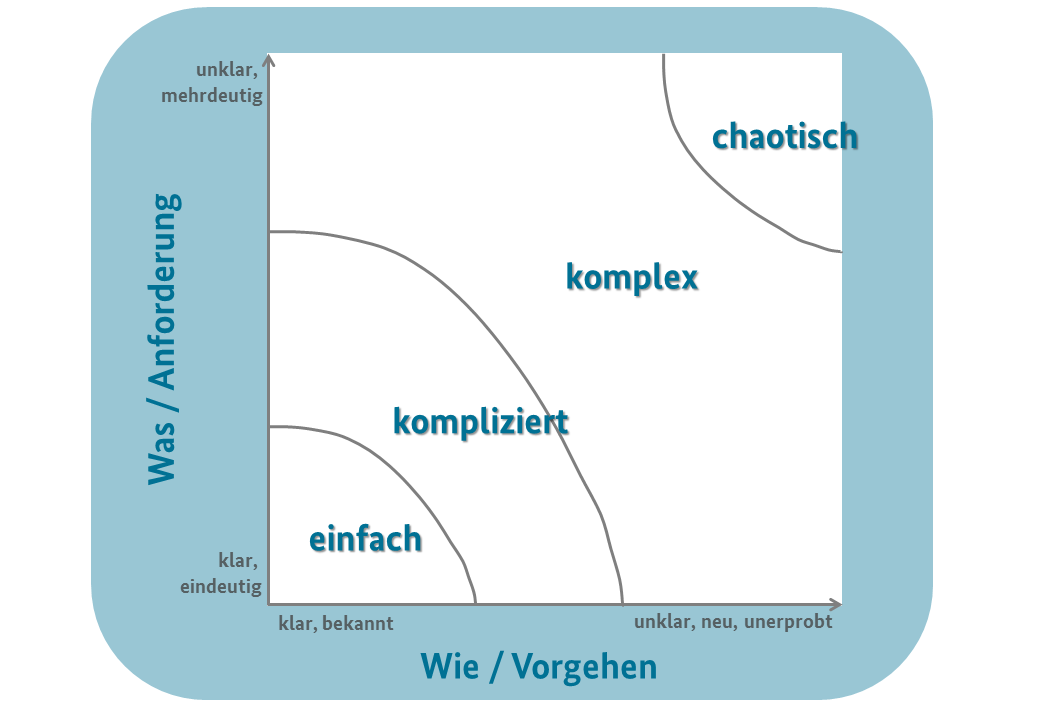
\includegraphics[width=6.24cm, height=4.32cm]{StaceyMatrix}
\caption{Stacey Matrix (\url{https://www.bva.bund.de/DE/Services/Behoerden/Beratung/Beratungszentrum/GrossPM/Wissenspool/_documents/Standardartikel/stda-stacey-matrix.html})}
\end{figure}

Im Bezug auf das geplante Projekt sind die Anforderungen noch nicht wirklich klar ausformuliert. Die Geschäftsführung hat eine Vision, eine grobe Idee und keinen klaren Katalog an sorgfältig definierten Anforderungen. Die Anforderungen sind also unklar.\\

Das Vorgehen an sich ist innerhalb des organisatorischen Ökosystems der Philetairus Immobilien GmbH unklar und unerprobt. Die IT Abteilung hat zuvor noch keine größeren Entwicklungsprojekte durchgeführt, daher ist auf diesem Gebiet wenig Erfahrung vorhanden und die Einbindung und  Einarbeitung der neuen Mitarbeiter kommt noch hinzu. Es gibt keine Erfahrungswerte innerhalb des Unternehmens auf die zurückgegriffen werden könnte, das Vorgehen ist daher unklar und unerprobt.\\

Basierend auf diesen Parametern ist dieses Projekt als Komplex einzuschätzen, daher ist ein agiles Vorgehen ratsam um der bestehenden Unklarheit möglichst flexibel zu begegnen und während des Projektes die geeigneten Methoden und Techniken zu erarbeiten. Für ein klassisches Vorgehen wäre eine langwierige Vorbereitungsphase notwendig, in der die genauen Anforderungen ermittelt werden müssten, bevor das Projekt überhaupt starten könnte.\\

Ein weiterer Vorteil des agilen Vorgehens in diesem Fall besteht in der zuvor beschriebenen Iterativen und Inkrementellen Vorgehensweise. So kann in regelmäßigen Abständen der Fortschritt überprüft werden und gegebenenfalls Anpassungen und Ergänzungen an den Anforderungen vorgenommen werden. Prinzipiell wäre das auch bei einem traditionellen Ansatz möglich, allerdings ist es dort mit einem größeren Aufwand verbunden einmal fixierte Projektanforderungen zu ändern .\\

Diese Flexibilität steht in direktem Zusammenhang mit der engen Einbindung der (in diesem Fall unternehmensinternen) Auftraggeber, die typisch für agiles Projektmanagement ist. Während die Auftraggeber bei klassischen Vorgehen konkrete Anforderungen zu Beginn des Projektes definieren und diese dann entweder zum Ende (oder zu festgelegten Meilensteinen) prüfen und abnehmen, stehen der Auftraggeber (oder dessen Vertreter) bei agilen Vorgehen in ständiger Kommunikation mit dem Entwicklerteam, prüfen die Zwischenprodukte (Inkremente) und beteiligen sich aktiv an der Anpassung und Aktualisierung der Anforderungen (zum Beispiel über das Product Backlog, siehe ~\ref{subsec:productGoalBacklog}).\\

Zu der Flexibilität des Vorgehens und des geringen Aufwands der Projektvorbereitung kommt ein weiterer Vorteil hinzu - die vergleichsweise hohe Anzahl der neuen Mitarbeiter, die durch die Erweiterung der IT Abteilung hinzugekommen sind. Diese sind noch nicht vollständig in die Unternehmensstrukturen integriert, auch hier bietet der agile Ansatz den Vorteil, da er auf flache Hierachien und Zusammenarbeit auf Augenhöhe setzt und die neuen Mitarbeiter somit schneller in das Ökosystem integriert werden können.\\

Aus diesen Gründen wurde der Entschluss gefasst, das Projekt agil anzugehen. Allerdings gab es von Seiten der Geschäftsleitungen einige Bedenken bezüglich eines rein agilen Vorgehens, weshalb weitere Überlegungen zur Projektstruktur angestellt wurden.\\